\documentclass{uebblatt}

\newcommand{\cont}{\mathrm{cont}}
\newcommand{\http}{http:/\kern-.2em/\kern-0.03em}

\begin{document}

\maketitle{11}{}

\begin{aufgabe}{2+m}{Rechenregeln für Ideale in dedekindschen Bereichen}
Bestätige folgende Rechenregeln für Ideale in einem dedekindschen Bereich.
\begin{enumerate}
\item $\aaa \cap (\bbb + \ccc) = (\aaa \cap \bbb) + (\aaa \cap \ccc).$
\item $\aaa + (\bbb \cap \ccc) = (\aaa + \bbb) \cap (\aaa + \ccc).$
\end{enumerate}
\end{aufgabe}

\begin{aufgabe}{3}{Inhalt von Polynomen über dedekindschen Bereichen}
Sei~$A$ ein Ring. Der \emph{Inhalt} eines Polynoms~$f = a_0 + \cdots +
a_m X^m \in A[X]$ ist das Ideal~$\cont(f) \defeq (a_0,\ldots,a_m)$.
Zeige, dass im Fall dass~$A$ ein dedekindscher Bereich ist, die
Rechenregel~$\cont(fg) = \cont(f) \cdot \cont(g)$ für Polynome~$f$ und~$g$
über~$A$ gilt.
\end{aufgabe}

\begin{aufgabe}{m+2}{Chinesischer Restsatz in dedekindschen Bereichen}
Seien~$\aaa_1,\ldots,\aaa_n$ Ideale in einem Ring~$A$.
\begin{enumerate}
\item Zeige, dass die untenstehende Sequenz von~$A$-Moduln genau dann exakt ist
(wie sehen die Abbildungen aus?), wenn für alle~$x_1,\ldots,x_n \in A$
folgendes gilt: Das System~$x \equiv x_i \pmod{\aaa_i}, i = 1,\ldots,n$ besitzt
eine Lösung~$x \in A$, falls~$x_i \equiv x_j \pmod{\aaa_i + \aaa_j}$ für
alle~$i,j$.
\[ A \longrightarrow \bigoplus_i A/\aaa_i \longrightarrow \bigoplus_{i < j} A/(\aaa_i
+ \aaa_j). \]
\item Zeige, dass diese Sequenz exakt ist, falls~$A$ ein dedekindscher Bereich
ist.
\end{enumerate}
\end{aufgabe}

\begin{aufgabe}{m}{Fit mit topologischen Räumen? Hausdorff macht Spaß}
Sei~$X$ ein topologischer Raum. Zeige, dass~$X$ genau dann hausdorffsch ist,
wenn die Diagonale~$\Delta \defeq \{ (x,x) \,|\, x \in X \}$ von~$X \times X$
abgeschlossen ist.
\end{aufgabe}

\centering
\rotatebox{90}{\tiny\sffamily \qquad\qquad \http www.smbc-comics.com/?id=3131}
\href{http://www.smbc-comics.com/?id=3131}{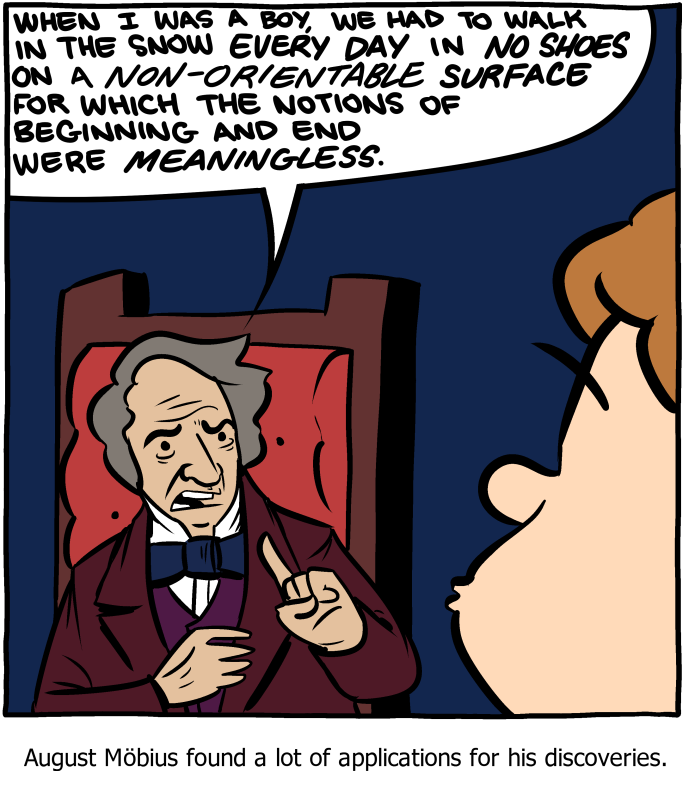
\includegraphics[scale=0.25]{images/smbc-moebius}}

\end{document}

* Zariski-Kotangentialraum ausrechnen.
